\section{Method}
\label{sec:method}

In this section we recall the theoretical framework of the \textit{Multi-Channel Variational Autoencoder} (MCVAE) developed in previous works \citep{Antelmi2018, Antelmi2019}, which we now enrich with the novel capability of dealing with missing views.
In \S~\ref{ssec:generative_model} and \S~\ref{ssec:derivation} we adopt new symbols and change the derivation of the cost function to conveniently set the problem of data modeling when some views are missing, and to make the relationships among views explicit and clear.
In \S~\ref{ssec:parameterization} we briefly recall the main parametric functions adopted later in our experiments with missing data.
In \S~\ref{ssec:optimization} we finally propose the new optimization scheme allowing not to discard observations with partially missing views, which is the main contribution of this work.

\subsection{Generative Model}
\label{ssec:generative_model}

Let $\Dcal = \set{D_d}_{d=1}^D$ be a collection of $D$ independent datasets, where each dataset $D_d = \set{\xdn}_{n=1}^{N_d}$ is composed by $N_d$ independent data-points (\eg subjects in the case of medical imaging datasets).
Every dataset $D_d$ is associated with a total number of $V_d$ available views
(\eg sets of clinical scores, imaging derived phenotypes extracted from multiple imaging modalities, \ldots),
and we assume that each data-point $\xdn = \set{\xdnv}_{v=1}^{V_{d,n}}$ is composed by $V_{d,n}$ views,
where $V_{d,n} \leq V_d$.
With the latest inequality we account for data-points with an arbitrary number of missing views.

For each view $\xdnv$ we propose the following generative latent variable model:
\begin{equation}\label{eq:model}
\begin{aligned}
&\z_{d,n} \sim \p{\z}, \\  % = \GaussStdDim{l} \\
&\xdnv \sim \p{\xdnv|\z_{d,n},\thetab_v},  % = \Gauss{\mub_c(\z)}{\Sigmab_c(\z) | \thetab_c}
\qquad \textnormal {for} \; v \; \textnormal{in} \; 1 \ldots V_{d,n} \leq V_d,
\end{aligned}
\end{equation}
where $\pz$ is a prior distribution for the latent variable $\z_{d,n}$ commonly shared by the $V_{d,n}$ views, and
where the likelihood functions $\p{\xdnv|\z_{d,n},\thetab_v}$ belong to a family of distributions parametrized by $\thetab_v$, which represents the view-specific generative parameters shared among all datasets.

\subsection{Variational Inference}
\label{ssec:derivation}

The exact solution to the inference problem is given by the posterior $\p{\z|\set{\xdnv,\thetab_v}_{v=1}^{V_{d,n}}}$, that is not generally computable analytically.
We can nevertheless look for its approximation $\qz$ through \textit{Variational Inference} \citep{Blei2017}.
By introducing the latent variational approximation $\qz$, we can derive the lower bound on the marginal log-likelihood for a single data-point as follows:
\begin{equation}\label{eq:LB}
\begin{aligned}
\ln \p{\xdnv|\thetab_v} &= \ln \int \p{\xdnv|\z, \thetab_v} \p{\z} \; d\z \\
                        &= \ln \int \frac{\qz}{\qz} \p{\xdnv|\z, \thetab_v} \p{\z} \; d\z \\
                        &= \ln \EE{\qz}{\frac{\p{\xdnv|\z, \thetab_v} \p{\z}}{\qz}} \\
                        &\geq \EE{\qz}{\ln \p{\xdnv|\z, \thetab_v}} - \KL{\qz}{\pz}.
\end{aligned}
\end{equation}
To derive the last line of \eqnref{eq:LB} we leverage on the \textit{Jensen's inequality} applied to the logarithm function, and collect the result into a new expectation term and in the Kullback-Leibler divergence term ($\kl$).

We define the distribution function $\qz$ to depend on a specific dataset $d$, data-point $n$, and view $w$, such that:
\begin{equation}\label{eq:q}
\begin{aligned}
\qz = q_{d,n,w}(\z) = \q{\z|\x_{d,n,w}, \phib_w},
\end{aligned}
\end{equation}
where $\phib_w$ represents the view-specific variational parameters shared among all datasets.
To force a link among views, we impose the inequality \eqnref{eq:LB} to hold for any $w$ in $1 \ldots V_{d,n}$.
To do so, we average the right hand side of \eqnref{eq:LB} across the $V_{d,n}$ views and rewrite \eqnref{eq:LB} as follows:
\begin{equation}\label{eq:newLB}
\begin{aligned}
% \ln \p{\xdnv|\thetab_v} &\geq \underbrace{\frac{1}{V_{d,n}} \sum_{w=1}^{V_{d,n}}
%   \EE{q_{d,n,w}(\z)}{\ln \p{\xdnv|\z, \thetab_v}}
% - \KL{q_{d,n,w}(\z)}{\pz}}_{\LBn}. \\
\ln \p{\xdnv|\thetab_v} \geq \LBdnv = \frac{1}{V_{d,n}} \sum_{w=1}^{V_{d,n}} \LBdnvw,
\end{aligned}
\end{equation}
where
\begin{equation}\label{eq:LBdnvw}
\begin{aligned}
\LBdnvw = \EE{q_{d,n,w}(\z)}{\ln \p{\xdnv|\z, \thetab_v}} - \KL{q_{d,n,w}(\z)}{\pz}
\end{aligned}
\end{equation}
is the lower bound associated to the data-point $\xdn$ when its view $v$ is predicted from its view $w$.
In \figref{fig:architecture} we sketch the model structure induced by \eqnref{eq:LBdnvw}.

\begin{figure}[htbp]
\centering
\includegraphics[width=\columnwidth]{./tex/fig/architecture.pdf}
\caption{
General variational framework for our multi-view model.
For every pair of views $v$ and $w$ there is a prediction path $v \leftarrow w$ composed by two learnable functions: the encoding distribution $\q{\z|\xb_w, \phib_w}$ and the decoding likelihood $\p{\xb_v|\z, \thetab_v}$.
Parameters $\phib_w$ and $\thetab_v$ are optimized through \eqnref{eq:argmax} to maximize the likelihood of our generative model under the encoding distributions, and at the same time minimize the Kullback-Leibler distance between every encoder and the prior $\pz$.
To leave the notation uncluttered, in this representation we dropped the dataset index $d$ and data-point $n$ used in the text.
}
\label{fig:architecture}
\end{figure}


\subsection{Parameterization}
\label{ssec:parameterization}

With the right choice of the functional form of $\q{\z|\x_{d,n,w}, \phib_w}$, $\pz$, and $\p{\xdnv|\z, \thetab_v}$, the \rhs\ of \eqnref{eq:newLB} becomes amenable to computation and maximization, yielding to the maximization of the \lhs, also known as the model evidence.
Of course, the choice for the likelihood function $\p{\xdnv|\z, \thetab_v}$ depends not only on pure computability considerations but also on the nature of the view $\xdnv$.
For example it can be parametrized as a multivariate Gaussian in the case of continuous data (\ie imaging derived phenotypes), as a Bernoulli likelihood for dichotomic data, as a Categorical likelihood for categorical data, \textit{etc}.

In general, the prior distribution $\pz$ is the  multivariate Gaussian distribution $\Gausstd$.
The same family of distributions is also commonly used for the variational and likelihood functions, such that respectively:
\begin{alignat}{4}
\label{eq:encoder}
\q{\z|\xdnw, \phib_w}  &= \mathcal{N} \left( \mub = \mathbf{V}_w^{(\mu)} \xdnw \right. &&{}; &&\left.\Sigmab = \diagp{\mathbf{V}_w^{(\sigma)} \xdnw} \right), \\
\label{eq:decoder}
\p{\xdnv|\z,\thetab_v} &= \mathcal{N} \left( \mub = \mathbf{G}_v^{(\mu)} \zb \right. &&{} ; &&\left.\Sigmab = \diagp{\mathbf{g}_v^{(\sigma)}} \right),
\end{alignat}
where the moments $\mub$ and $\Sigmab$ are linear transformations of the conditioning variables.
Here, $\thetab_v = \{\mathbf{G}_v^{(\mu)}, \mathbf{g}_v^{(\sigma)}\}$ and $\phib_w=\{\mathbf{V}_w^{(\mu)}, \mathbf{V}_w^{(\sigma)}\}$ are the parameters to be optimized.
A non-linear parameterization can be as well used, for example in the form of deep neural networks.

In the literature we can also find the following alternative parameterization for the posterior distribution:
\begin{equation}
\label{eq:dropout_posterior}
    q_{d,n,w}(\z) = \Gauss{\mub = \mathbf{V}_w^{(\mu)} \xdnw}{\Sigmab = \diagp{\sqrt{\alphab} \odot \mub^2}},
\end{equation}
which is known as \textit{dropout posterior} \citep{Kingma2015}.
The dropout parameter $\alphab$ has components $\alpha_i = \nicefrac{p_i}{1-p_i}$ linked to the probability $p_i$ of dropping out the $i$-th latent variable component \citep{Wang2013}.
It has been shown that the association of this dropout posterior with a log-uniform prior distribution $\pz$ leads to sparse and interpretable models \citep{Antelmi2019,Molchanov2017}.

\subsection{Optimization}
\label{ssec:optimization}

Assuming independent observations, the marginal log-likelihood in the left hand side of \eqnref{eq:newLB} can be summed up over all the datasets, data-points, and views.
As a consequence, inference on the model generative parameters $\thetab = \set{\thetab_v}$ and variational parameters $\phib = \set{\phib_w}$ can be achieved by solving the maximization problem:
\begin{equation}\label{eq:argmax}
\begin{aligned}
\hat{\thetab}, \hat{\phib} &= \underset{\thetab, \phib}{\argmax} \sum_{d,n,v} \LBdnv \\
                           &= \underset{\thetab, \phib}{\argmax} \sum_{d,n,v} \frac{1}{V_{d,n}} \sum_{w=1}^{V_{d,n}} \LBdnvw.
\end{aligned}
\end{equation}
We use Algorithm \ref{alg:optim} to solve \eqnref{eq:argmax}.
\begin{algorithm} % enter the algorithm environment
\caption{Model parameters optimization} % give the algorithm a caption
\label{alg:optim} % and a label for \ref{} commands later in the document
\begin{algorithmic} % enter the algorithmic environment
	\Require Initialize the model parameters $\phib, \thetab$. Set the optimizer learning rate.
	\While{$\phib, \thetab$ not converged}
		\State $\lb \leftarrow 0$
		\For{every dataset $d \in D$}
			\For{every datapoint $n \in N_d$}
				\For{every \textit{decoding} view $v \in V_{d,n}$}
					\State $\lb_v \leftarrow 0$
					\For{every \textit{encoding} view $w \in V_{d,n}$}
						\State Accumulate the cost of decoding $\xdnv$ through the encoder $q_{d,n,w}(\z)$:
						\State $\lb_v \leftarrow \lb_v + \EE{q_{d,n,w}(\z)}{\ln \p{\xdnv|\z, \thetab_v}} - \KL{q_{d,n,w}(\z)}{\pz}$.
					\EndFor
					\State Average the decoding cost and accumulate it in the total cost $\lb$:
					\State $\lb \leftarrow \lb + \frac{1}{V_{d,n}} \lb_v$.
				\EndFor
			\EndFor
		\EndFor
		\State $\thetab, \phib = \optim(\phib, \thetab, \nabla_{\phib} \lb, \nabla_{\thetab} \lb)$. \textit{Adam} optimizer used to maximie $\lb$.
	\EndWhile
\end{algorithmic}
\end{algorithm}
% \begin{algorithm} % enter the algorithm environment
% \caption{Calculate $y = x^n$} % give the algorithm a caption
% \label{alg1} % and a label for \ref{} commands later in the document
% \begin{algorithmic} % enter the algorithmic environment
%     \REQUIRE $n \geq 0 \vee x \neq 0$
%     \ENSURE $y = x^n$
%     \STATE $y \Leftarrow 1$
%     \IF{$n < 0$}
%         \STATE $X \Leftarrow 1 / x$
%         \STATE $N \Leftarrow -n$
%     \ELSE
%         \STATE $X \Leftarrow x$
%         \STATE $N \Leftarrow n$
%     \ENDIF
%     \WHILE{$N \neq 0$}
%         \IF{$N$ is even}
%             \STATE $X \Leftarrow X \times X$
%             \STATE $N \Leftarrow N / 2$
%         \ELSE[$N$ is odd]
%             \STATE $y \Leftarrow y \times X$
%             \STATE $N \Leftarrow N - 1$
%         \ENDIF
%     \ENDWHILE
% \end{algorithmic}
% \end{algorithm}

The summation in \eqnref{eq:argmax} is done for every dataset $d$ along all the available data-points $n$ and their specific views $v$.
We note that batching data-points with common views can speed up the computation by reducing the number of second level \textit{for} loop iterations in Algorithm \ref{alg:optim}.
If missing, a particular view $v$ will be simply not accounted for that specific observation, without having to discard all the other views that can still contribute to optimize \eqnref{eq:argmax}.
The presence of at least one common view among datasets acts as a link and allows the information to flow through all the datasets to the other views.
In \figref{fig:model} we show the learning scheme of our model in a simple case with four views and one common view between batches.

\begin{figure*}[tb]
\centering
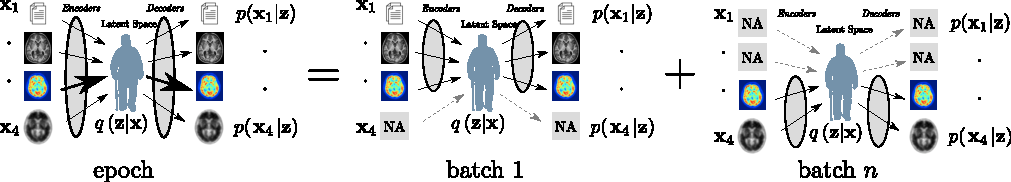
\includegraphics[width=\textwidth]{./tex/fig/model.pdf}
\caption{
Multi-view learning scheme in the presence of missing not available (NA) data.
Arrows represent trainable functions used as network encoders and decoders.
The contribution of datapoints to the model learning is reduced in.
}
\label{fig:model}
\end{figure*}


We observe that this model extends the Multi-Channel VAE \citep{Antelmi2019}, which is a multi-view extension of the VAE \citep{Kingma2013,Rezende2014}.
The authors of \cite{Antelmi2019} propose a multi-view generative model where they require all the observation in the training set to have all the available views, hence limited to model one dataset at a time (in the case of datasets with different views), after having discarded incomplete observations in that dataset.
We address this limitation by allowing missing views in the training set for some observations.
Similarly to \cite{Antelmi2019}, the trained model can estimate missing views from the available ones through the formula:
\begin{equation}\label{eq:reconstruction}
\begin{aligned}
\hat\xb_{d,n,v} = \frac{1}{V_{d, n}-1} \sum_{w=1, \,w\neq v}^{V_{d, n}} \EE{q_{d,n,w}(\z)}{\p{\xdnv|\z, \thetab_v}}.
\end{aligned}
\end{equation}

% \subsection{Architectures}
% So far we have explicitly modeled a one-to-one correspondence between encoding and decoding views, which is the focus of our work.
% This makes our model part of the family of the auto-encoders, where the model acts as a identity transformation between the input and the output.
% Other architectures are nevertheless possible.
% Let's consider, for example, the case where a many-to-one relationship exists between many encoding views and one decoding view.
% In this case, we can consider our model as a multi-view regressor, if the output likelihood function models a continuous variable, or a multi-view classifier in the case of a finite discrete output.
% In general, there may be an $m$-to-$n$ relationship, with partially overlapping views among $m$ input views and $n$ output views.
% Investigating the properties of all the possible architectures is beyond the scope of this work.

